% This is samplepaper.tex, a sample chapter demonstrating the
% LLNCS macro package for Springer Computer Science proceedings;
% Version 2.21 of 2022/01/12
%
\documentclass[runningheads]{llncs}
%
\usepackage[T1]{fontenc}
% T1 fonts will be used to generate the final print and online PDFs,
% so please use T1 fonts in your manuscript whenever possible.
% Other font encondings may result in incorrect characters.


% tightlist command for lists without linebreak
\providecommand{\tightlist}{%
  \setlength{\itemsep}{0pt}\setlength{\parskip}{0pt}}


% Pandoc citation processing
\newlength{\cslhangindent}
\setlength{\cslhangindent}{1.5em}
\newlength{\csllabelwidth}
\setlength{\csllabelwidth}{3em}
\newlength{\cslentryspacingunit} % times entry-spacing
\setlength{\cslentryspacingunit}{\parskip}
% for Pandoc 2.8 to 2.10.1
\newenvironment{cslreferences}%
  {}%
  {\par}
% For Pandoc 2.11+
\newenvironment{CSLReferences}[2] % #1 hanging-ident, #2 entry spacing
 {% don't indent paragraphs
  \setlength{\parindent}{0pt}
  % turn on hanging indent if param 1 is 1
  \ifodd #1
  \let\oldpar\par
  \def\par{\hangindent=\cslhangindent\oldpar}
  \fi
  % set entry spacing
  \setlength{\parskip}{#2\cslentryspacingunit}
 }%
 {}
\usepackage{calc}
\newcommand{\CSLBlock}[1]{#1\hfill\break}
\newcommand{\CSLLeftMargin}[1]{\parbox[t]{\csllabelwidth}{#1}}
\newcommand{\CSLRightInline}[1]{\parbox[t]{\linewidth - \csllabelwidth}{#1}\break}
\newcommand{\CSLIndent}[1]{\hspace{\cslhangindent}#1}


\usepackage{graphicx}
% Used for displaying a sample figure. If possible, figure files should
% be included in EPS format.
%
% If you use the hyperref package, please uncomment the following two lines
% to display URLs in blue roman font according to Springer's eBook style:
\usepackage{hyperref}
\usepackage{color}
\renewcommand\UrlFont{\color{blue}\rmfamily}


\begin{document}


\title{CytokineFinder: identifying disease associated cytokines}
%
% If the paper title is too long for the running head, you can set
% an abbreviated paper title here
%
\author{Jeffrey Tang\inst{1,2}\orcidID{0000-1111-2222-3333} \and Amrit
Singh\inst{1,2}\orcidID{1111-2222-3333-4444}}


\authorrunning{F. Author et al.}
% First names are abbreviated in the running head.
% If there are more than two authors, 'et al.' is used.
%

\institute{Department of Anesthesiology, Pharmacology \& Therapeutics,
The University of British Columbia, Vanouver, Canada \and Centre for
Heart Lung Innvation, St.~Paul's Hosital, Vanouver, Canada}

\maketitle              % typeset the header of the contribution
%
\begin{abstract}
The abstract should briefly summarize the contents of the paper in
150--250 words.

\keywords{First keyword \and Second keyword \and Another keyword}

\end{abstract}

\hypertarget{introduction}{%
\section{Introduction}\label{introduction}}

\begin{itemize}
\tightlist
\item
  importance of identifying driver cytokines
\item
  mention limitations in publicly available cytokine data
\item
  state hypothesis: using gene expression data we can identify the
  driver cytokines of disease
\end{itemize}

\hypertarget{methods}{%
\section{Methods}\label{methods}}

\hypertarget{public-cytokine-data-curation}{%
\subsection{public cytokine data
curation}\label{public-cytokine-data-curation}}

\begin{itemize}
\tightlist
\item
  cytokine stimulations
\item
  anti-cytokine treatment
\item
  studies with paired gene-expression and protein data
\end{itemize}

\hypertarget{study-data}{%
\subsection{study data}\label{study-data}}

\begin{itemize}
\tightlist
\item
  asthma gene expression data
\item
  validate with cytokien protein levels
\end{itemize}

\hypertarget{cytoknefinder}{%
\subsection{cytokneFinder}\label{cytoknefinder}}

\begin{itemize}
\tightlist
\item
  add workflow diagram of study (figure 1)
\item
  briefly describe each method; but add more details of each method in
  the supplement
\end{itemize}

\hypertarget{benchmarking-analysis}{%
\subsection{benchmarking analysis}\label{benchmarking-analysis}}

\hypertarget{data-analysis-of-study-data}{%
\subsection{data analysis of study
data}\label{data-analysis-of-study-data}}

\begin{itemize}
\tightlist
\item
  apply best method to study data
\end{itemize}

\hypertarget{results}{%
\section{Results}\label{results}}

\hypertarget{benchmarking-figure-2}{%
\subsection{Benchmarking (figure 2)}\label{benchmarking-figure-2}}

\begin{itemize}
\tightlist
\item
  impact of annotations
\item
  which method+ann works best
\end{itemize}

\hypertarget{study-results}{%
\subsection{study results}\label{study-results}}

\begin{itemize}
\tightlist
\item
  patient demographics
\item
  cytokine finder results with study data
\item
  hypothesis testing for significant cytokines
\end{itemize}

\hypertarget{discussion}{%
\section{Discussion}\label{discussion}}

\hypertarget{a-subsection-sample}{%
\subsection{A Subsection Sample}\label{a-subsection-sample}}

Please note that the first paragraph of a section or subsection is not
indented. The first paragraph that follows a table, figure, equation
etc. does not need an indent, either.

Subsequent paragraphs, however, are indented.

\hypertarget{sample-heading-third-level}{%
\subsubsection{Sample Heading (Third
Level)}\label{sample-heading-third-level}}

Only two levels of headings should be numbered. Lower level headings
remain unnumbered; they are formatted as run-in headings.

\hypertarget{sample-heading-fourth-level}{%
\paragraph{Sample Heading (Fourth
Level)}\label{sample-heading-fourth-level}}

The contribution should contain no more than four levels of headings.
Table~\ref{tab:table} gives a summary of all heading levels.

\begin{table}

\caption{\label{tab:table}Table captions should be placed above the tables.}
\centering
\begin{tabular}[t]{r|r}
\hline
temperature & pressure\\
\hline
0 & 0.0002\\
\hline
20 & 0.0012\\
\hline
40 & 0.0060\\
\hline
60 & 0.0300\\
\hline
80 & 0.0900\\
\hline
100 & 0.2700\\
\hline
\end{tabular}
\end{table}

\noindent Displayed equations are centered and set on a separate line.

\begin{equation}
x + y = z
\end{equation}

Please try to avoid rasterized images for line-art diagrams and schemas.
Whenever possible, use vector graphics instead (see
Fig.~\ref{fig:fig1}).

\begin{figure}
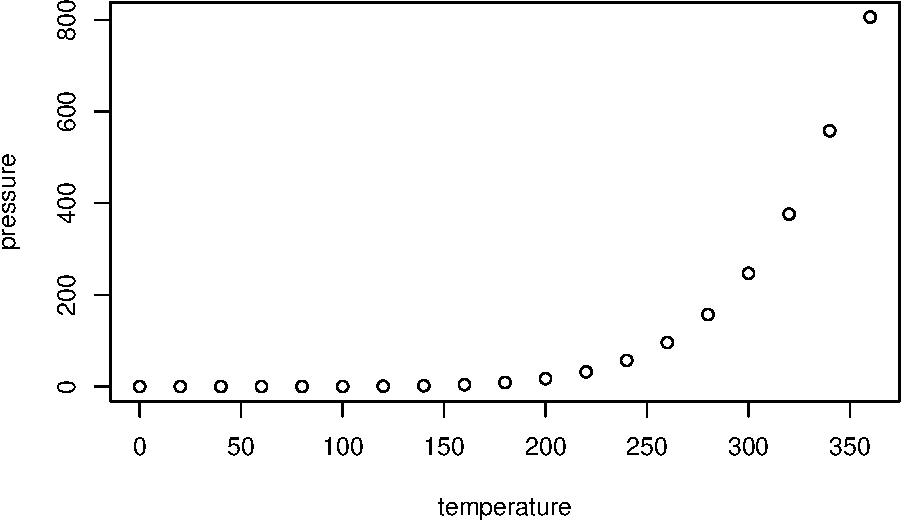
\includegraphics{manuscript_files/figure-latex/fig1-1} \caption{A figure caption is always placed below the illustration. Please note that short captions are centered, while long ones are justified by the macro package automatically.}\label{fig:fig1}
\end{figure}

\begin{theorem}
This is a sample theorem. The run-in heading is set in bold, while the
following text appears in italics. Definitions, lemmas, propositions,
and corollaries are styled the same way.

\end{theorem}

The environments `definition', `lemma', `proposition', `corollary',
`remark', and `example' are defined in the LLNCS documentclass as well.

\begin{proof}
Proofs, examples, and remarks have the initial word in italics, while
the following text appears in normal font.

\end{proof}

For citations of references, use {[}1{]}. Multiple citations are grouped
{[}2{]}, {[}3{]}.

\hypertarget{acknowledgements}{%
\subsubsection{Acknowledgements}\label{acknowledgements}}

Please place your acknowledgments at the end of the paper, preceded by
an unnumbered run-in heading (i.e.~3rd-level heading).

\hypertarget{references}{%
\section*{References}\label{references}}
\addcontentsline{toc}{section}{References}

\hypertarget{refs}{}
\begin{CSLReferences}{0}{0}
\leavevmode\vadjust pre{\hypertarget{ref-Nuncio2011}{}}%
\CSLLeftMargin{1. }%
\CSLRightInline{Nuncio, M., Luis, A.J., Yuan, X.: {Topographic
meandering of Antarctic Circumpolar Current and Antarctic Circumpolar
Wave in the ice-ocean-atmosphere system}. Geophysical Research Letters.
38, 1--5 (2011).
https://doi.org/\href{https://doi.org/10.1029/2011GL046898}{10.1029/2011GL046898}.}

\leavevmode\vadjust pre{\hypertarget{ref-Levitus2012}{}}%
\CSLLeftMargin{2. }%
\CSLRightInline{Levitus, S., Yarosh, E.S., Zweng, M.M., Antonov, J.I.,
Boyer, T.P., Baranova, O.K., Garcia, H.E., Locarnini, R.A., Mishonov,
A.V., Reagan, J., Seidov, D.: {World ocean heat content and thermosteric
sea level change (0-2000), 1955-2010}. Geophysical Research Letters. 39,
1--5 (2012).
https://doi.org/\href{https://doi.org/10.1029/2012GL051106}{10.1029/2012GL051106}.}

\leavevmode\vadjust pre{\hypertarget{ref-Raphael2004}{}}%
\CSLLeftMargin{3. }%
\CSLRightInline{Raphael, M.N.: {A zonal wave 3 index for the Southern
Hemisphere}. Geophysical Research Letters. 31, 1--4 (2004).
https://doi.org/\href{https://doi.org/10.1029/2004GL020365}{10.1029/2004GL020365}.}

\end{CSLReferences}

%
% ---- Bibliography ----



\end{document}
